\documentclass[11pt,openany]{article}
\usepackage{geometry}
\geometry{
	letterpaper,
	margin=1in
}
\usepackage{blindtext}
\usepackage{tikz,tcolorbox,tikz-3dplot}
\usepackage{pgfplots}
\usepgfplotslibrary{fillbetween}
\usepackage{xcolor}
\usepackage{amsfonts}
\usepackage{hyperref} 
\usepackage{indentfirst}
\usepackage{graphicx}
\usepackage{caption}
\usepackage{subcaption}
\usepackage[normalem]{ulem}
\usepackage [english]{babel}
\usepackage [autostyle, english = american]{csquotes}
\usepackage{appendix}

\usepackage[ruled,linesnumbered]{algorithm2e}
\SetKwComment{Comment}{/* }{ */}
\DontPrintSemicolon 
\usepackage{tabularx}
\usepackage{amsmath,amssymb}
\usepackage{mathtools}
\usepackage{makecell}
\graphicspath{ {./images/} }
\usepackage{enumitem}
\usepackage{soul}
\usepackage{mathtools}
\usepackage{wrapfig}
\usepackage{mathrsfs}
\usepackage{centernot}
\usepackage{amsthm}
\usepackage{listings}
%\usepackage{biblatex}
%\addbibresource{bibliograph.bib}
\usepackage{microtype}
\usepackage{pagenote}
\usepackage{array}
\usepackage{xparse}

\tcbuselibrary{theorems}

\definecolor{codegreen}{rgb}{0,0.6,0}
\definecolor{codegray}{rgb}{0.5,0.5,0.5}
\definecolor{codepurple}{rgb}{0.58,0,0.82}
\definecolor{backcolour}{rgb}{0.95,0.95,0.92}

\lstdefinestyle{mystyle}{
	backgroundcolor=\color{backcolour},   
	commentstyle=\color{codegreen},
	keywordstyle=\color{magenta},
	numberstyle=\tiny\color{codegray},
	stringstyle=\color{codepurple},
	basicstyle=\ttfamily\footnotesize,
	breakatwhitespace=false,         
	breaklines=true,                 
	captionpos=b,                    
	keepspaces=true,                 
	numbers=left,                    
	numbersep=5pt,                  
	showspaces=false,                
	showstringspaces=false,
	showtabs=false,                  
	tabsize=2
}

\lstset{style=mystyle}
%% End notes to be printed as sections at the
%% end of each chapter.
\renewcommand*{\notedivision}{\section*{\notesname}}
\renewcommand*{\pagenotesubhead}[1]{}

%\newcommand*{\exercises}{\section*{\exercisename}}
%%%%%%%%%%%%% For customising the endnote markers. Comment these out if you don't want them.
% To prefix each note number with the chapter number
\renewcommand{\thepagenote}{\thechapter-\arabic{pagenote}}

% To have a slightly different formatting for the endnote numbers in the text -- smaller text, sans-serif, square brackets
\renewcommand\notenumintext[1]{\space{\footnotesize\sffamily[FN-#1]}}

% To have a slightly different formatting for the endnote numbers in the notes section. Just the square brackets and sans-serif; normal size.
\renewcommand\notenuminnotes[1]{{\sffamily[FN-#1] }}
% If you want a different name/heading for the end notes
\renewcommand{\notesname}{End Notes}
\newcommand{\exercisename}{Exercises}
\newcounter{thatonetheorem}
\newcounter{exercisecounter} % continuity of exercises in a section
\newenvironment{exerciselist}{
	\begin{enumerate}
		\setcounter{enumi}{\value{exercisecounter}}
	}{
		\setcounter{exercisecounter}{\value{enumi}}
	\end{enumerate}
}
\newenvironment{thatonethmlist}{
	\begin{enumerate}
		\setcounter{enumi}{\value{thatonetheorem}}
	}{
		\setcounter{thatonetheorem}{\value{enumi}}
	\end{enumerate}
}
\newcommand*{\exercises}{\section*{\exercisename}}

\newcommand\todo{\textcolor{red}{\textbf{TODO: }}}
%%%%%%%%%%%%% End customisation
\newcommand{\reals}{\mathbb{R}}
\newcommand\defeq{\mathrel{\stackrel{\makebox[0pt]{\mbox{\normalfont\tiny def}}}{=}}}
\makeatletter
\renewcommand*\env@matrix[1][*\c@MaxMatrixCols c]{%
  \hskip -\arraycolsep
  \let\@ifnextchar\new@ifnextchar
  \array{#1}}
\makeatother

\newcounter{thmcounter} % continuity of theorem

\newcommand{\definition}[2]{\addtocounter{thmcounter}{1}
\begin{tcolorbox}[title=Definition {\thesection}.{\arabic{thmcounter}} ({#1}),colframe=black]
		{#2}\end{tcolorbox}


}
\newcommand{\proposition}[1]{
	\addtocounter{thmcounter}{1}
	\begin{tcolorbox}[title=Proposition {\thesection}.{\arabic{thmcounter}},colframe=red!50!blue!20!white,colback=red!35!blue!10!white, coltitle=black]{#1}\end{tcolorbox}

}
\newcommand{\theorem}[2]{
\addtocounter{thmcounter}{1}
\begin{tcolorbox}[title=\color{black}Theorem {\thesection}.{\arabic{thmcounter}} ({#1}),colframe=red!40,colback=red!5!white]{#2}\end{tcolorbox}
	
}
\newcommand{\lemma}[1]{
\addtocounter{thmcounter}{1}
\begin{tcolorbox}[title=\color{black}Lemma {\thesection}.{\arabic{thmcounter}},colframe=blue!40,colback=blue!5!white]{#1}\end{tcolorbox}
	
}
\newcommand{\example}[1]{\addtocounter{thmcounter}{1}\begin{tcolorbox}[title=Example {\thesection}.{\arabic{thmcounter}},colframe=yellow!20!white,colback=yellow!10!white,coltitle=black]{#1}\end{tcolorbox}


}
\newcommand{\corollary}[1]{	\addtocounter{thmcounter}{1}\begin{tcolorbox}[]{Corollary {\thesection}.{\arabic{thmcounter}}: {#1}}\end{tcolorbox}
	

}


%%% Eliseu's fix for theorem numbering

% Definition
\NewTcbTheorem[number within=section, use counter=thmcounter]{adefinition}{Definition}{
	colframe=black, 
	separator sign none, 
	description delimiters parenthesis}{def}
% Proposition
\NewTcbTheorem[number within=section, use counter=thmcounter]{aproposition}{Proposition}{
	colframe=red!50!blue!20!white,colback=red!35!blue!10!white, coltitle=black,
	separator sign none, 
	description delimiters parenthesis}{prop}
% Theorem
\NewTcbTheorem[number within=section, use counter=thmcounter]{atheorem}{Theorem}{
	colframe=red!40,colback=red!5!white, coltitle=black,
	separator sign none, 
	description delimiters parenthesis}{thm}

% Lemma
\NewTcbTheorem[number within=section, use counter=thmcounter]{alemma}{Lemma}{
	colframe=blue!40,colback=blue!5!white, coltitle=black,
	separator sign none, 
	description delimiters parenthesis}{lemma}
% Example
\NewTcbTheorem[number within=section, use counter=thmcounter]{aexample}{Example}{
	colframe=yellow!20!white,colback=yellow!10!white,coltitle=black,
	separator sign none, 
	description delimiters parenthesis}{ex}
% Corollary
\NewTcbTheorem[number within=section, use counter=thmcounter]{acorollary}{Corollary}{
	separator sign none, 
	description delimiters parenthesis,
	coltitle=black,
	attach title to upper={:\ }}{cor}


%%% Eliseu's fix for backwards compatibility with Chi's macros

\let\olddefinition\definition
\let\oldproposition\proposition
\let\oldtheorem\theorem
\let\oldexample\example
\let\oldcorollary\corollary
\let\oldlemma\lemma

\renewcommand{\definition}[3][\relax]{\ifx\relax#1\olddefinition{#2}{#3}\else \begin{adefinition}{#2}{#1} #3 \end{adefinition} \fi}
\renewcommand{\proposition}[2][\relax]{\ifx\relax#1\oldproposition{#2}\else \begin{aproposition}{}{#1} #2 \end{aproposition} \fi}
\renewcommand{\theorem}[3][\relax]{\ifx\relax#1\oldtheorem{#2}{#3}\else \begin{atheorem}{#2}{#1} #3 \end{atheorem} \fi}
\renewcommand{\example}[2][\relax]{\ifx\relax#1\oldexample{#2}\else \begin{aexample}{}{#1} #2 \end{aexample} \fi}
\renewcommand{\corollary}[2][\relax]{\ifx\relax#1\oldcorollary{#2}\else \begin{acorollary}{}{#1} #2 \end{acorollary} \fi}
\renewcommand{\lemma}[2][\relax]{\ifx\relax#1\oldlemma{#2}\else \begin{alemma}{}{#1} #2 \end{alemma} \fi}
\newtheorem*{remark}{Remark}
\newtheorem*{notation}{Notation}
%\newcommand{\exercises}{\section*{\exercisename}}
%% THIS LINE IS MANDATORY
\makepagenote

\newcommand{\newsection}{\setcounter{thmcounter}{0}}
%\ref{def:label}, \ref{prop:label}, \ref{thm:label}, \ref{ex:label}, \ref{cor:label}.
% \setcounter{thmcounter}{0}
% \begin{atheorem}[foor}{bar}{label} or use square brackets before the function, like 
\setcounter{section}{-1}
\usepackage{titling}
\predate{}
\postdate{}
\date{}
\title{EE 495 Game Theory and Networked Systems}
%\author{Chi Li}
\begin{document}
\maketitle
\section{Syllabus}
\newsection
All logistics are on canvas.

Randy Berry: Office L352.

There are no required texts for the class. There are some references (4) that are suggested on Canvas. 
\subsection*{Prereqs}
\begin{enumerate}
    \item No prior knowledge on game theory is required.
    \item Mathematical background is required. Linear algebra, probability, optimization, mathematical maturity.
\end{enumerate}
\subsection*{Grades}
\begin{itemize}
    \item Midterm: in class, $35\%$
    \item Final project: $35\%$
    \item Problemsets: $30\%$
\end{itemize}
\begin{atheorem}{}{}
    Randy is a chill professor.
\end{atheorem}
\section{Lecture 1: Introduction to Game Theory}
\newsection
\definition{Game Theory}{
    Game theory is the study of interactions of \textit{multiple strategic agents}.
}
Features of game theory:\begin{itemize}
    \item More than one decision makers.
    \item Each agent makes decisions to maximize self-interest.
    \item These \textbf{agents} are players of the `game', and can be people, firms, countries (in political science), AI-agents etc.
\end{itemize}

\example{
    The following are examples of `games':\begin{itemize}
        \item 2 people playing chess. Their incentives do not align because each player wants to checkmate the other.
        \item 2 firms competing in a market. They are selling the similar items and are trying to price their items to get a larger market share.
        \item 4 countries competing to maximize GDP.
    \end{itemize}
}

The other component of this course is network systems.
\example{
    The following are examples of network systems:\begin{itemize}
        \item Communication network. 
        \item Electricity network.
        \item Transportation network.
    \end{itemize}
}
We will use these as examples to illustrate the concepts in game theory. However, the same theory can extend into the other games.
We want to model and analyze games. People are complicated to model, and our models are simplifications of reality. We need to understand what assumptions are made for each models to apply analysis. 

\subsection*{Basic Game Model}
\definition[basicgame]{Basic Game Model}{
    A \textbf{strategic form game} $G$ consists of the following elements:\begin{enumerate}
        \item The set of agents/players $R$, usually enumerated $R=\{1,2,3,\ldots, n\}$.
        \item For every $r\in R$, the action set of player $r$ $S_r$. If $\left|\bigsqcup_r S_r\right|<\infty$, we call the game a \textbf{finite game}.
        \item For every $r\in R$, a payoff function $\pi_r:\otimes_{r'} S_{r'}\to \reals$. Each agent $r$ wants to maximize $\pi_r$. 
    \end{enumerate}
}
That means, there is only one round of this game, and everyone makes the same decision all at once.
\begin{remark}
    The action set can also be called the strategic set.
\end{remark}
\begin{notation}
    The ordered set of everyone's actions except $r$ is \[
        \overline{s_{-r}}=(s_1,s_2,\ldots, s_{r-1},s_{r+1},\ldots,s_n).
    \]
    Therefore player $r$ is actually maximizing \[
    \pi_r(s_r,\overline{s_{-r}}).
    \]
    The second part of this function is outside of $r$'s control.
\end{notation}

\example{
    Consider two Internet Service Providers (ISPs)
    \begin{center} 
    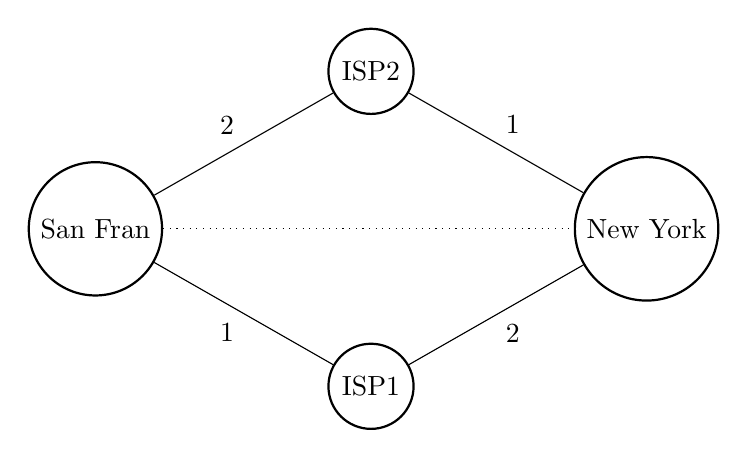
\begin{tikzpicture}
        \begin{scope}[every node/.style={circle,thick,draw}]
        \node (a) at (0,0) {San Fran};
        \node (b) at (7,0){New York};
        \node (c) at (3.5,2){ ISP2};
        \node (d) at (3.5,-2){ ISP1};
        \end{scope}
        \draw [dotted] (a) --  (b);
        \draw (a) -- node[midway, below left]{1}(d) -- node[midway, below right]{2}(b);
        \draw (a)-- node[midway, above left]{2} (c) --node[midway, above right]{1}(b);
    \end{tikzpicture}\end{center}

    They have peered i.e. no charge to send traffic to each other. 
    There is 1MB of traffic to ISP 1 customers in NY. There is 1mB of traffic to ISP 2 in SF. Each ISP will incur the cost of usage of the two (respective) edges connected to it, per mB of traffic.
    Here,\begin{align*}
        R&=\{1,2\}\\
        S_r&=\{\textrm{near},\textrm{far}\}, 
    \end{align*}
    that is, each ISP can decide whether to send the traffic directly or through the other ISP.
}
We can represent this as a matrix 
\iffalse
  ISP1 \ ISP2  near far

near (-4,-4) (-1,-5)

far (-5,-1) (-2,-2)


\fi
\begin{center}
    \begin{tabular}{|c|c c|} 
        \hline
        ISP 1\textbackslash ISP2 & near & far \\ 
        \hline
        near & (-4,-4) & (-1,-5) \\ 
        \hline
        far & (-5,-1) & (-2,-2)\\
        \hline
    \end{tabular}
\end{center}

\definition[dominant]{Dominant action}{
    An Action is $s_r^*$ is \textbf{weakly dominant} if \[
    \pi_r(s_r^*,\overline{s_{-r}})\geq\pi_r(s_r,\overline{s_{-r}})
    \]
    for all $s_r\neq s_r^*$, and any $\overline{s_{-r}}$.
    If inequality is strict, then the action is \textbf{strictly dominant}.
}
\corollary{
    If the game has a strictly dominant action for each player, this will give a unique dominant strategy equilibrium.
}
\example{
    Consider the game with the reward matrix:
    \begin{center}
        \begin{tabular}{|c|c c c|} 
            \hline
            1\textbackslash 2 & L & M & R \\ 
            \hline
            U & (1,0) & (2,-1) & (1,2) \\ 
            \hline
            D & (0,3) & (1,4)& (0,1)\\
            \hline
        \end{tabular}
    \end{center}
    There is no dominant action for player 2, but there is a dominant action (U) for player 1. Therefore, player 2 can rationally assume that player 1 does not play D. Under this assumption, player 2 has a dominant strategy of (R).
}
\example[techorkellog]{
    Alice and Bob want to get lunch together
    Consider the game with the reward matrix:
    \begin{center}
        \begin{tabular}{|c|c c|} 
            \hline
            1\textbackslash 2 & Tech&Kellog \\ 
            \hline
            Tech & (2,3) & (1,1)\\ 
            \hline
            Kellog & (1,1)&(3,2)\\
            \hline
        \end{tabular}
    \end{center}
    There is no dominant action for each player. This is known as a coordination game, it is better to follow what the other player chooses.
}
\definition[nasheq]{Nash Equilibrium}{
    A strategy profile $(s_1^*,\ldots, s_n^*)$ is a \textbf{Nash equilibrium} if \[
    \pi_r(s^*_r,s^*_{-r})\geq\pi_r(s_r,s^*_{-r})
    \]
    for each agent $r$, $s_r\in S_r$.

    In other words, no player benefits from unilateral deviations.
}
In the case of Example \ref{ex:techorkellog}, the two Nash equilibria are when both players pick the same place to eat. However, there are no dominant strategies! Even if we made the matrix 
\begin{center}
    \begin{tabular}{|c|c c|} 
        \hline
        1\textbackslash 2 & Tech&Kellog \\ 
        \hline
        Tech & (5,5) & (1,1)\\ 
        \hline
        Kellog & (1,1)&(2,2)\\
        \hline
    \end{tabular}
\end{center}
there will still be two Nash equilibria, even though the (5,5) outcome is much better than the other (2,2) - some are better than others.

\proposition{
    A dominant strategy equilibrium is a Nash equilibrium.
}
\begin{proof}
    By definition.
\end{proof}
\begin{aexample}{Attacker Defender}{attackdefend}
    
    Consider the reward matrix
    \begin{center}
        \begin{tabular}{|c|c c|} 
            \hline
            Attacker\textbackslash User & A&B \\ 
            \hline
            A & (1,0) & (0,1)\\ 
            \hline
            B & (0,1)&(1,0)\\
            \hline
        \end{tabular}
    \end{center}
    The attacker always wants to choose the channel with the user, but the user wants a different channel. In this case, there is no Nash equilibrium (either the attacker can move to the user channel or the user move away from the attacker channel).
\end{aexample}
\subsection*{Next Time}
Mixed strategies, thm: finite game with randomized strategies always have nash equilibria.
\end{document}